\documentclass[11pt]{article}
\usepackage[utf8]{inputenc}
\usepackage[portuguese, english]{babel}
\usepackage[T1]{fontenc}
\usepackage{subfigure} 
\usepackage{lmodern}
\usepackage{geometry}
\usepackage{authblk}
\usepackage{graphicx}
\usepackage{multicol}
\usepackage{multirow}
\usepackage{float} 
\usepackage{amsmath}

\newcommand\scalemath[2]{\scalebox{#1}{\mbox{\ensuremath{\displaystyle #2}}}}

\geometry{legalpaper, margin=1in}
\renewcommand{\arraystretch}{1.15}


\graphicspath{{../}}

\begin{document}


\title{\textbf{Circuit Theory and Electronics Fundamentals - T4}}
\author[1]{João D. Álvares}
\author[1]{João M. Teixeira}
\author[1]{Rui M. Martins}

\affil[1]{\textit{\normalsize{Instituto Superior Técnico, Av. Rovisco Pais 1, 1049-001 Lisboa}}}

\date{23th May 2021}
\maketitle

\renewenvironment{abstract}[1]
  {\bigskip\selectlanguage{#1}%
   \begin{center}\bfseries\abstractname\end{center}}
  {\par\bigskip}

\begin{abstract}{english}
    In this report, we focus on implementing a band-pass filter recurring to an operational amplifier (OP-AMP) which must provide a voltage gain of $40dB$ and a signal's central frequency of $1kHz$. To build the circuit, we had to consider not only the circuit's efficiency, but also its cost trying to minimize it. Having these in mind, we were able to build a circuit that allowed us to obtain a gain of (...) and a central frequency of (...). This culminated in a merit score of 
\end{abstract}

\begin{abstract}{portuguese}
    Neste relatório propôs-se a construção e estudo de um filtro passa-banda recorrendo-se, para tal, a um amplificador operacional (AMP-OP) que almejava alcançar um ganho de $40dB$ e uma frequência central para o sinal de saída de $1kHz$. Na construção do circuito teve-se em conta não apenas a consecução destes objetivos, mas também a tentativa de manter um custo total do circuito reduzido. Tendo isto em conta, construiu-se um circuito que permitiu obter um ganho de (...) e uma frequência central de (...). Estes valores culminaram, finalmente, num mérito de (...)
\end{abstract}
\tableofcontents
\addcontentsline{toc}{section}{\listtablename}
\listoftables
\addcontentsline{toc}{section}{\listfigurename}
\listoffigures
\cleardoublepage

\section{Introduction}
The main goal of this laboratory assignment is to explore different circuit analysis methods and to compare the results obtained with the results given by the \textit{Ngspice} simulation. For the theoretical analysis, the circuit will be analysed using mesh and nodal methods (both result from the Kirchoff's Laws) -  and the equations resulting from these methods will be solved using \textit{Octave}. On the other hand, the circuit simulation will be made, as said above, with \textit{Ngspice}. The analysed circuit can be seen in Fig. \ref{fig:esquema}.

\begin{figure}[h]
    \centering
    \includegraphics[width = 0.7\linewidth]{esquema.pdf}
        \caption{\textit{Circuit analysed. It consists, essentially, in a circuit with 4 essential meshes, 8 nodes and 11 branches (in which we count 7 resistors, 2 voltage sources - one of them controlled by the current $I_C$ - and 2 current sources - one independent and one dependent, controlled by the voltage $V_b$ as it can be seen in the figure. The labels used in this figure will be used throughout this report.}}
    \label{fig:esquema}
\end{figure}

As a starting point to solve this circuit, some values of the symbolic variables presented in Fig. \ref{fig:esquema} were given and are presented in Table \ref{tab:initial_values}:

\begin{table}[H]
    \begin{minipage}{.5\textwidth}
      \centering
      \begin{tabular}{c|c}
        \hline
        \multicolumn{2}{c}{Resistors [$k\Omega$]}  \\
        \hline
        $R_1$ & 1.03994439216 \\
        $R_2$ & 2.07923431764 \\
        $R_3$ & 3.06168544529 \\
        $R_4$ & 4.09516986362 \\
        $R_5$ & 3.00136467001 \\
        $R_6$ & 2.03324628446 \\
        $R_7$ & 1.02216788331
      \end{tabular}
    \end{minipage}
    \begin{minipage}{.5\textwidth}
      \centering
      \begin{tabular}{c|c}
        \hline
        \multicolumn{2}{c}{Currents [$mA$]}  \\
        \hline
        $I_d$ & 1.01674167773 \\
        \hline
        \hline
        \multicolumn{2}{c}{Voltages [$V$]}  \\
        \hline
        $V_a$ & 5.03847501972 \\
        \hline
        \hline
        \multicolumn{2}{c}{Dependent sources constants}  \\
        \hline
        $K_b$ & 7.01505323139 $mS$ \\
        $K_c$ & 8.37372457746 $k\Omega$
      \end{tabular}
    \end{minipage}
    \caption{Summary table with all the known values at the starting point}
    \label{tab:initial_values}
\end{table}
\section{Simulation Analysis and the Path for the Greater Good}

For this analysis, we used the default diode model available in \textit{Ngspice}, having then created the circuit presented in Fig. \ref{fig:bigscheme} (it was using Ngspice that we determined, in fact, what was the best circuit for our purposes). So, we used the following chain of thought in order to do what we did. In the envelope detector part, we took the limit as $R \rightarrow \infty$, which is the same as no current passing through there, which is the same as nothing being there. This drastically reduces our ripples, for then we do not need the resistance at all and the cost is 0. Of course this is slightly counterbalanced by the presence of the $10^{-6}$, in the merit calculation (\eqref{score}).  Knowing that the voltage ripples reduce to \eqref{eq:ripples}
\begin{equation}
    V_{ripple} = v_o(0) - v_o(T) = A \left(1 - e^{-\frac{T}{2RC}}\right)
    \label{eq:ripples}
\end{equation}
we can model very superficially the function that should describe this merit in terms of our components (\eqref{eq:approx}).

\begin{equation}
    f(R,C) = \frac{1}{(R+C)*A*\left(1 - e^{-\frac{T}{2RC}}+ 10^{-6}\right )}
    \label{eq:approx}
\end{equation}

From that, we can then plot what's the aspect of the function, shown in Fig. \ref{fig:plot}.

\begin{figure}[H]
    \centering
    \includegraphics[width = 0.85\linewidth]{cost.png}
        \caption{\textit{Merit approximated function. Plot obtained using GeoGebra3D}}
    \label{fig:plot}
\end{figure}

And thus we have the justification of our doings by removing the resistor. Then, we made use of the specifications of the non-linear part of the diodes and found that there is a very fortunate correlation between the amount of diodes in the voltage regulator and the ripples in the end voltage. What this means is that we can let go of the equation that says that $R2$ must be much greater than $rd$, for this is but a very rough approximation of the real life's diode behaviour. The only setback of this method is the stabilization time, but the merit does not take that into account, so we're good. This way, we used 31 diodes, for nonetheless we did not want to have an exaggerated stabilization time. WARNING: This will cause big differences between the theoretical analysis and the simulation. The model presented in class, when applied to Octave, will basically serve of nothing.

Finally, one found the values considered as the best to find an optimal merit score which are given by:

\begin{table}[H]
    \centering
    \begin{tabular}{|c|c|c|c|}
    \hline
        \textbf{Component} &  \textbf{Amount} & \textbf{Value} & \textbf{Cost}\\
        \hline
        \hline
        Resistors & 1 & $0.2k\Omega$ & 0.2\\
        \hline
        Capacitors & 1 &  $1.33\mu$F & 1.33\\
        \hline
        Diodes & 31+4 & - & 3.5 \\
        \hline
    \end{tabular}
    \caption{Components values shown in Fig. \ref{fig:bigscheme}.}
    \label{tab:tentativas}
\end{table}


\subsection{Cost and Merit Score}
Evaluating the merit, and knowing that the cost is given by \eqref{eq:cost}
\begin{equation}
    c = cost = 35 \cdot 0.1 + 0.2 + 1.33 =  4.85\text{MU}
    \label{eq:cost}
\end{equation}

Using the values obtained for $c$, $d$ and $r$, one can finally calculate the merit score obtained with this circuit (calculated using equation \eqref{score}), which allows one to get the following score:

\begin{equation}
    M = 3.31752e+02
\end{equation}

\subsection{Envelope Detector and Voltage Regulator output voltages}
To understand the role played by the envelope detector and the voltage regulator circuits in our circuit one plotted the results obtained for the output voltages in each one of them. So, starting by the plot obtained at the output terminals of the envelope detector circuit

\begin{equation}
    V = v_4
\end{equation}

Plotting this function:

\vspace{-140px}
\begin{figure}[H]
    \centering
    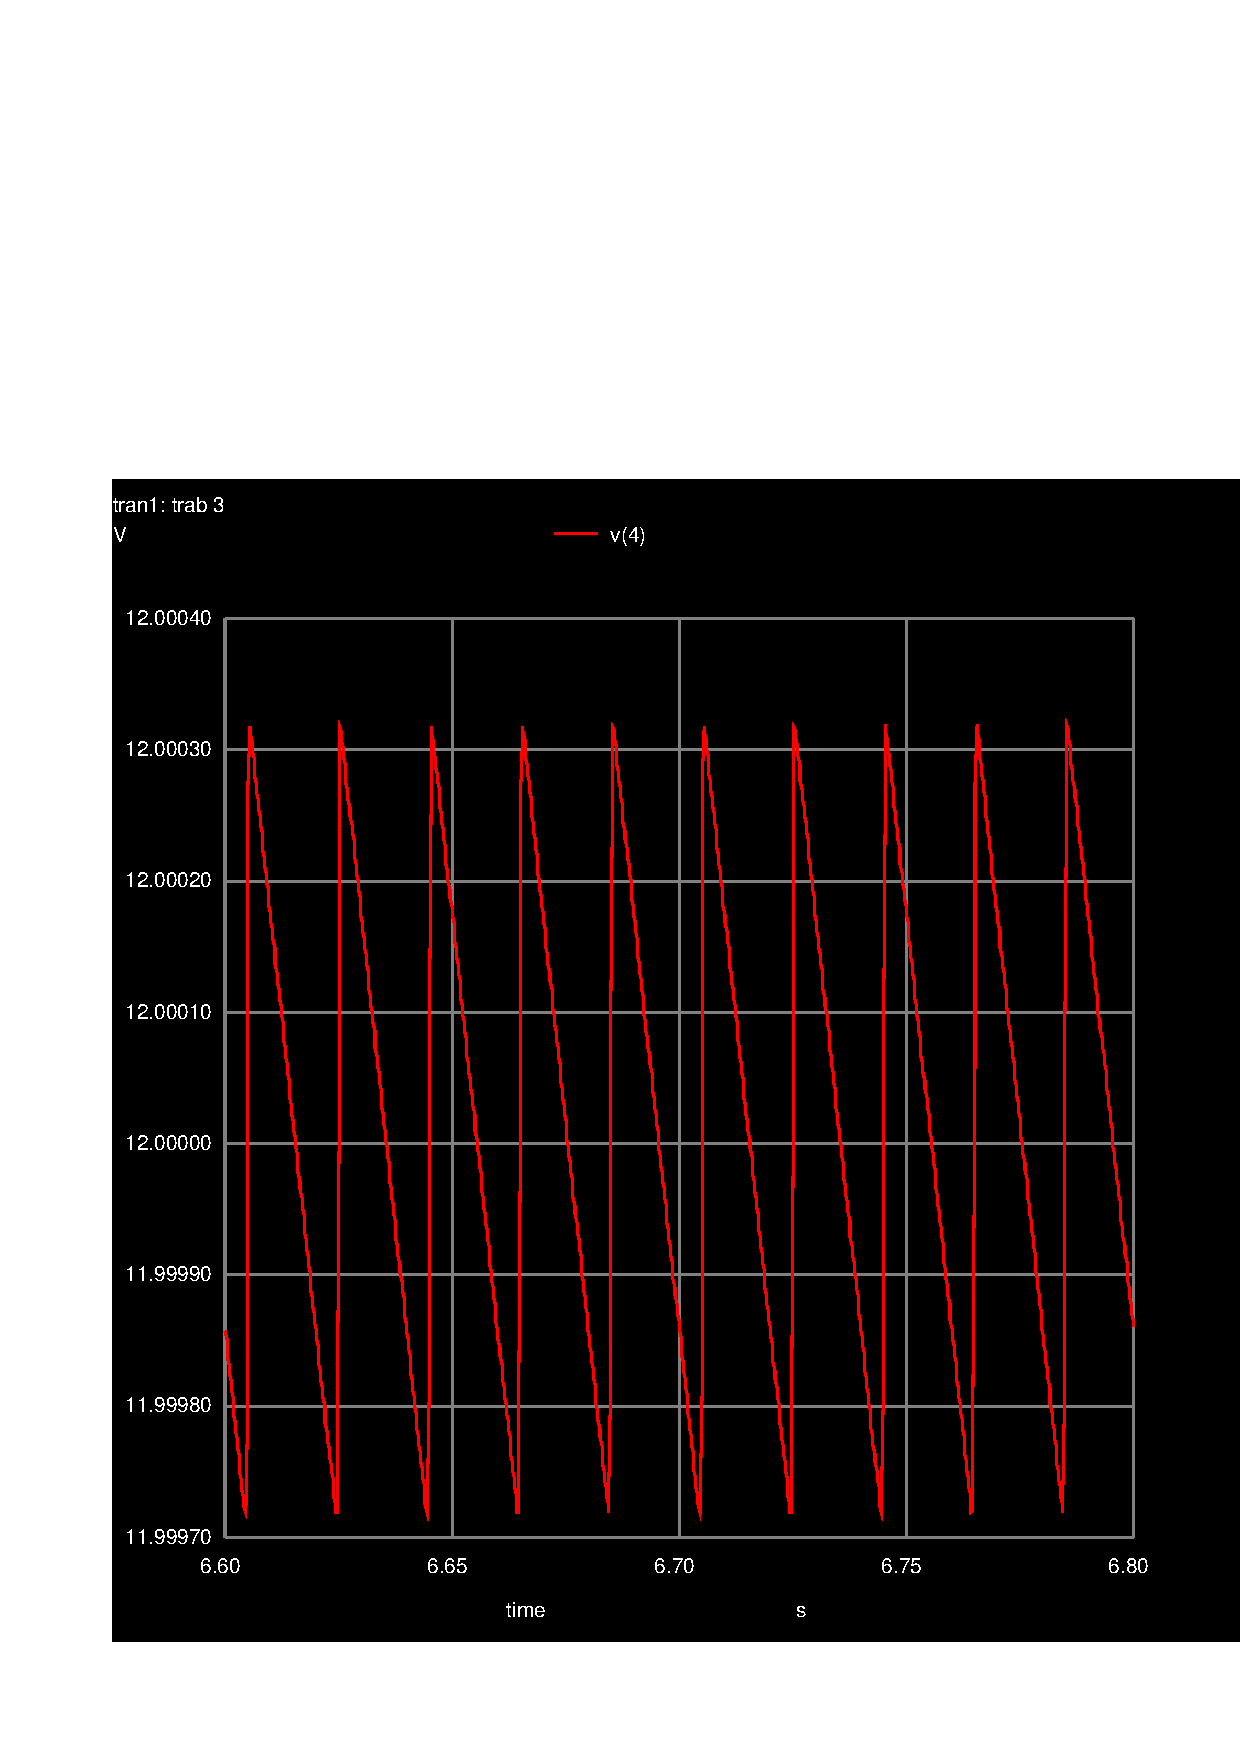
\includegraphics[width = 0.85\linewidth]{sim/antes.pdf}
    \vspace*{-10mm}
        \caption{\textit{Plot of the output voltage registered at the output terminals of the envelope detector circuit}}
    \label{fig:before}
\end{figure}

To plot the output voltage observed on the terminals of the voltage regulator circuit, one plotted the function given by

\begin{equation}
    V = v_5
\end{equation}

which allowed to get

\vspace{-140px}
\begin{figure}[H]
    \centering
    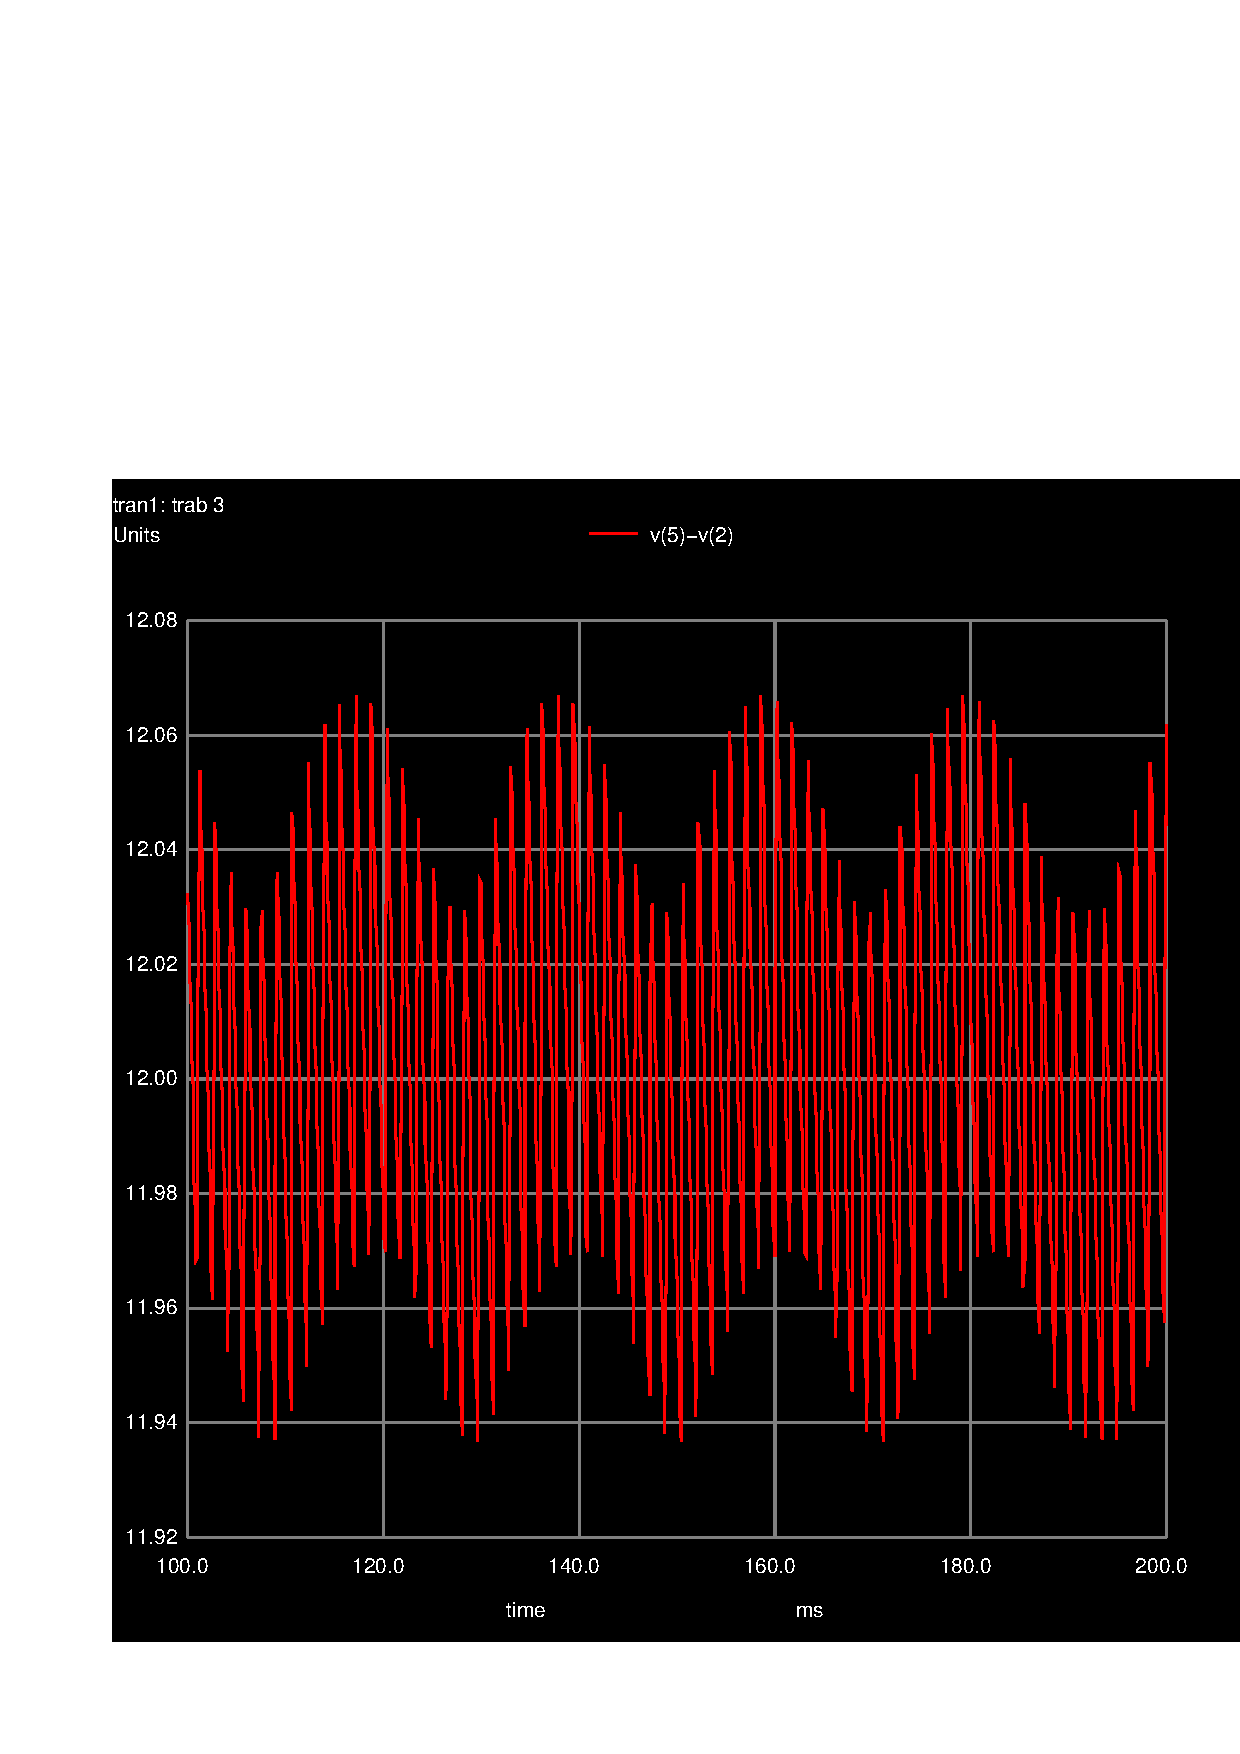
\includegraphics[width = 0.85\linewidth]{sim/zauzau.pdf}
    \vspace*{-10mm}
        \caption{\textit{Plot of the output voltage registered at the output terminals of the voltage regulator circuit}}
    \label{fig:zauzau}
\end{figure}

Comparing the two plots one can conclude that the plots are perfectly similar except on the $y$ axis scale. In fact, the difference between the two plots was caused by the action of our voltage regulator circuit. As the number of diodes was chosen to set an upper limit to the output voltage of the circuit to the desired value $V = 12V$ the difference registered between the two graphs only reflects the effect of that part of the circuit. And in fact, as one can see, the voltage regulator circuit is working as it is supposed to because the voltage that was intially oscillating around $14V$ is oscillating around $12V$ at the output terminals of the voltage regulator. This translates, numerically, into: INSERT HERE
\begin{equation}
    v_{6 average} = 
\end{equation}

\subsection{Plotting $v_o - 12$}
Finally, to conclude the simulation analysis (which one can antecipate that allowed to get precise and satisfactory results) and to better understand how the output voltage behaved next to the desired value of $V = 12V$, one plotted the function $V = v_o - 12$:

\vspace{-140px}
\begin{figure}[H]
    \centering
    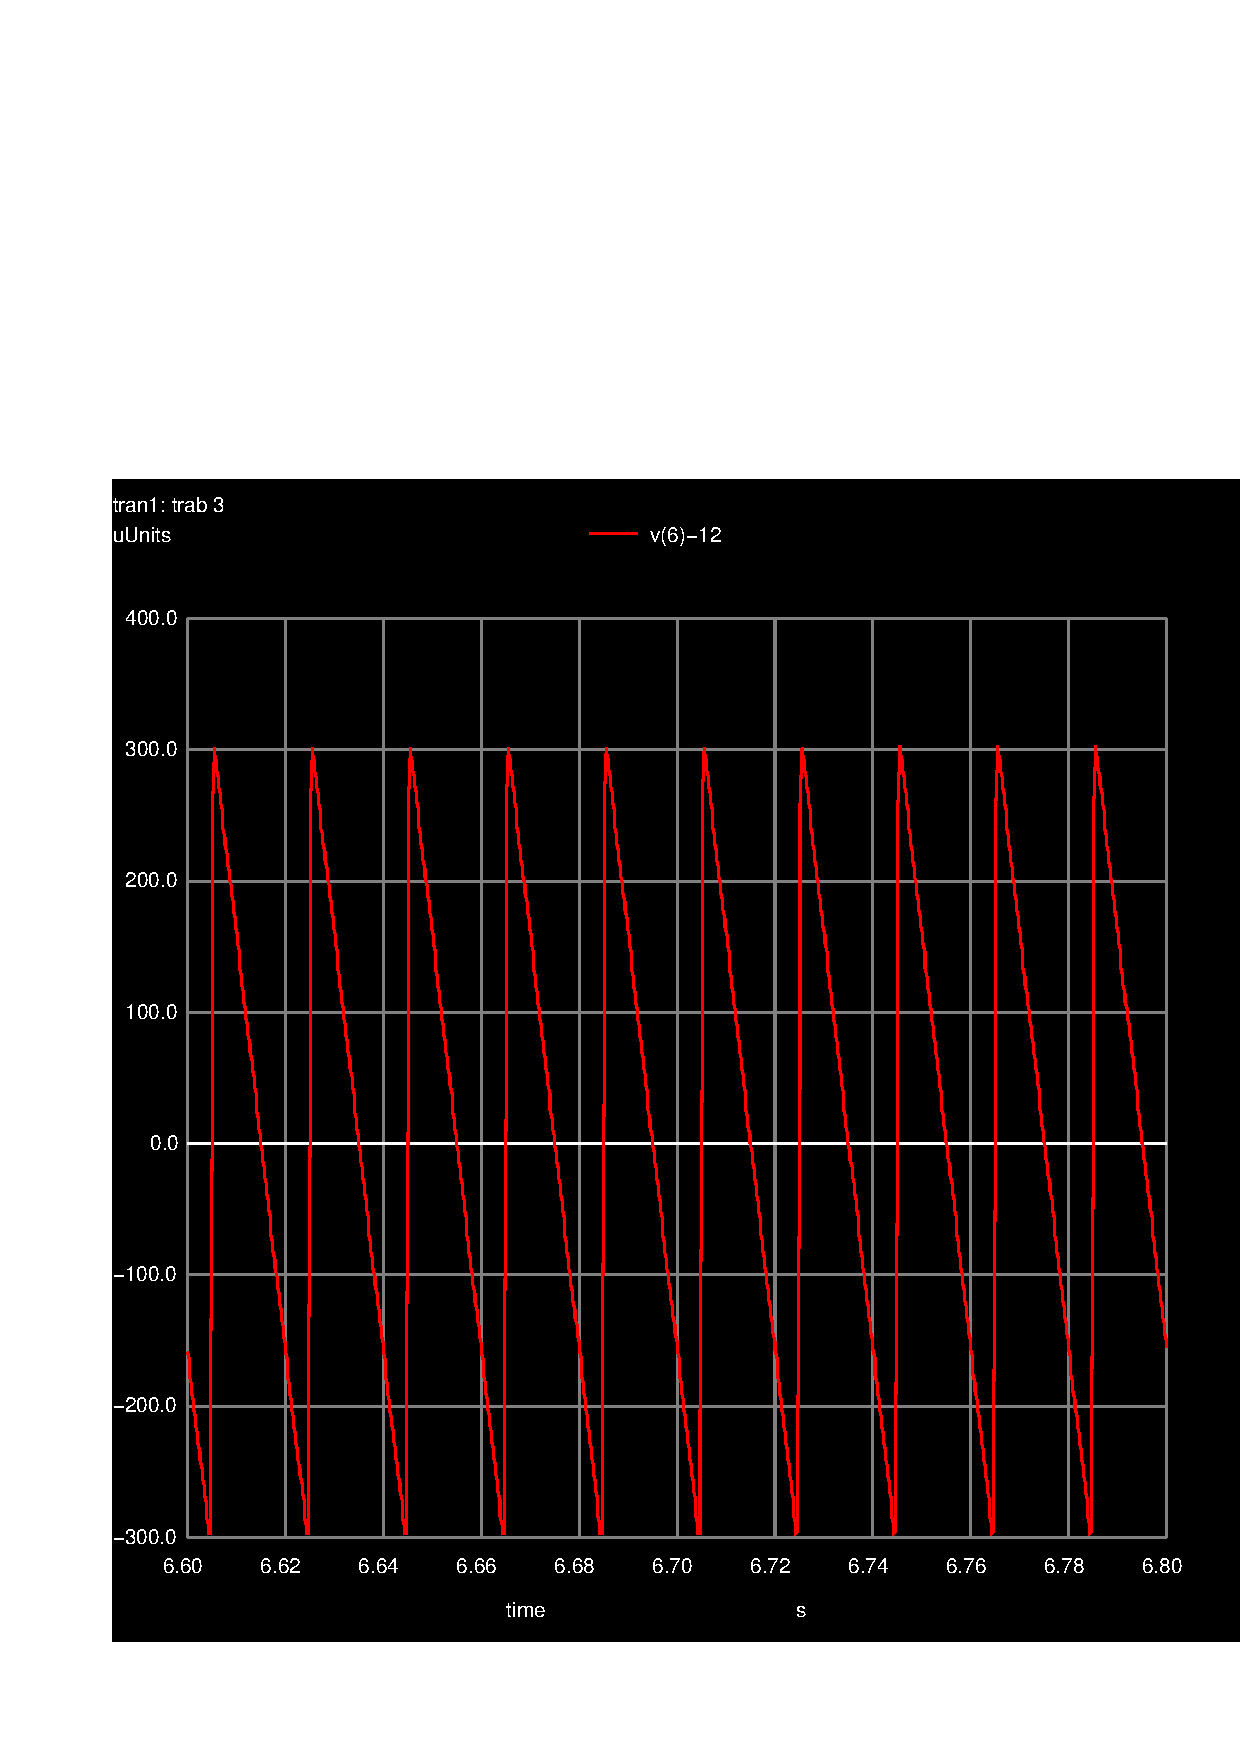
\includegraphics[width = 0.85\linewidth]{sim/deviation.pdf}
    \vspace*{-10mm}
        \caption{\textit{Plot of the difference between the circuit's output voltage and the desired voltage, $V=12V$}}
    \label{fig:dev}
\end{figure}

which, numerically, gives: INSERT HERE

\begin{equation}
    |v_6 - 12| = 
\end{equation}

\section{Theoretical Analysis}

In this analysis, we have some differences from the theoretical analysis for some of the standard parts of an AC-DC converter, those being the high number of diodes and the absence of the resistor in parallel with the capacitor.

Initially we started with a voltage source with the standard $\frac{230}{n}V$ and $50Hz$, in which $n$ was the one experimentally determined to produce the best merit in ngspice, in this case being $17.78988$, which produces an amplitude of $12.9287$.

The first part of the circuit to be analysed is the full-wave rectifier, which has a behaviour that is well described by the absolute value of the input wave, because the voltage is way bigger than $V_{ON}$ of the diode.

\begin{equation}
    V_{Full Wave} = \left|\frac{V_in}{n}\right|
    \label{eq:fullwave_mat}
\end{equation}

The next component is the capacitor has a envelope detector. The formula for calculating the envelope voltage in each period is 

\begin{equation}
    V_{envelope}=A\cos{(\omega t_{OFF})}e^{-\frac{t_{ON}-t_{OFF}}{RC}}
\end{equation}

with 

\begin{equation}
    t_{OFF}=\frac{1}{\omega}\arctan\left(\frac{1}{\omega R C}\right)
\end{equation}

But in our circuit we did not included the resistor so, with it being in parallel it will behave not as if the resistance is infinite but as the resistance that still exist in the diodes that is very high because we chose to use then even bellow $V_{ON}$. This being said, the resistance used in this formula for this specific analysis is $N r_d$, with $r_d$ as determined in the next section(\eqref{eq:rad_mat})

\begin{figure}[H]
    \centering
    \includegraphics[width = 0.85\linewidth]{mat/antes_mat.png}
        \caption{\textit{Signal as it exits the envelope detector according to the theoretical analysis.}}
    \label{fig:plot}
\end{figure}

The last part of the circuit is the voltage regulator, in our case it's a set of 31 diodes in series, all in parallel with the capacitor. In this analysis we followed the expected formulae, although, because of the heavy difference between simulation and theoretical analysis we can begin disprove the usage of these equations for higher number of diodes.

First we must understand the behavior of the diodes and the best way to understand it it through it's incremental resistance, it starts of as really high but than it decreases to more constant and low values and this change is exponential. That being said, the formula is the following. 

\begin{equation}
    r_d = \frac{\eta V_T}{I_S e^{\frac{V_D}{\eta V_T}}}
    \label{eq:rad_mat}
\end{equation}

\begin{figure}[H]
\hspace{-10mm}
  \subfigure[Current as function of voltage]{% 
    \includegraphics[width=.45\textwidth]{diode.png} \label{fig:diode} 
  } 
  \subfigure[Voltage as function of current]{% 
    \includegraphics[width=.5\textwidth]{diode_R.png} \label{fig:diode_R} 
  } 
  \caption{I-V characteristic of a diode} 
\end{figure}

In this figure we can both understand that the diodes have different regions depending on the voltage but, considering $R=\frac{dV}{dI}$, from the second figure we conclude that the resistance if extremely high for the OFF zone of the diode and it can be used as a high resistance instead of actual resistors.

with $\eta=1$, $V_T = 0.025V$, $I_S=10^-{14}$ and $V_D$ being the the voltage difference in each diode that the estimated as being the value in the input of the set of diodes divided by the number of diodes. And, as expected we obtained a big value that is 247280.745039$\Omega$. The biggest difference to the simulation analysis starts here: the high number of diodes seems to help stabilize the signal, but the following formula indicates that for high number of diodes and diode incremental resistance the oscillation after the voltage regulator must be the same as the one leaving the envelope detector

\begin{equation}
    v_o = \frac{N r_d}{N r_d + R}V_{envelope}
    \label{eq:v_o_mat}
\end{equation}

The only thing left to discuss is the DC component of this approximation for the voltage regulator which will be $V_{envelope}$ unless $V_{envelope}$ is bigger than $N V_{ON}$, but $V_{ON}$ is some value between $0.65$ and $0.7$ $k\Omega$ so it's upper limit with $N=31$ is way higher than any value in $V_{envelope}$, so the DC component is only change, and just a little, in the oscillation amplitude from the previous formula.


\begin{figure}[H]
    \centering
    \includegraphics[width = 0.85\linewidth]{mat/zauzau_mat.png}
        \caption{\textit{Output voltage according to the theoretical analysis.}}
    \label{fig:plot}
\end{figure}

\begin{figure}[H]
    \centering
    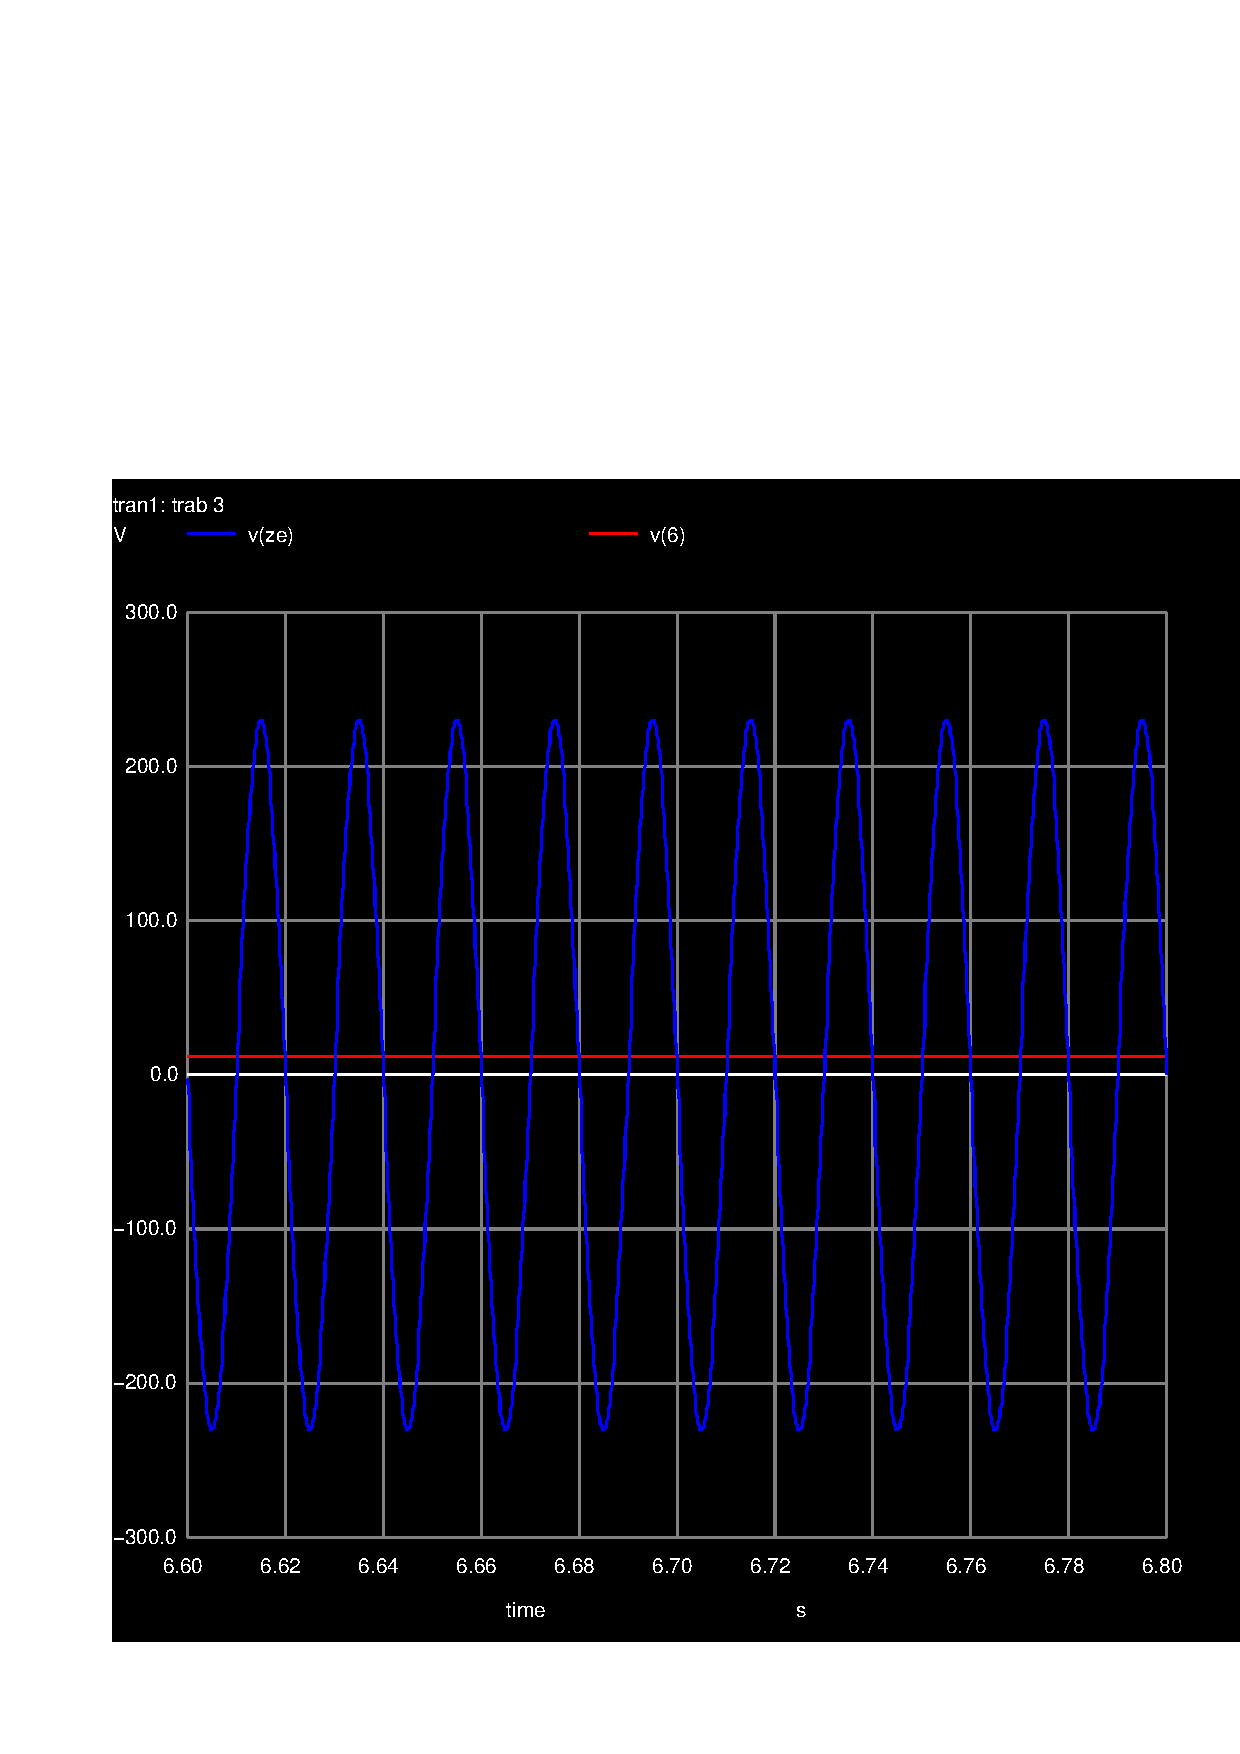
\includegraphics[width = 0.85\linewidth]{mat/acdc.png}
        \caption{\textit{Comparison between output and input voltage.}}
    \label{fig:plot}
\end{figure}

\begin{figure}[H]
    \centering
    \includegraphics[width = 0.85\linewidth]{mat/deviation_mat.png}
        \caption{\textit{Output signal minus the 12V goal.}}
    \label{fig:plot}
\end{figure}

With this output and the components used the final relevant values are the average of the signal \input{media}V, the ripple \input{ripple} and finally \input{merit}, but as we know the value of the average can be easily adjusted by n in the transformer so, removing that term, the corrected merit in the theoretical analysis is 1106.692837.
\section{Side by side comparison between both analysis results}
\label{sec:sidebyside}
\vspace{-85px}
\begin{figure}[H]
\hspace{-10mm}
  \subfigure[Theoretical analysis]{% 
    \includegraphics[width=.66\textwidth]{mat/gaindb.png}
  } 
  \hspace{-30px}
  \subfigure[Simulation analysis]{% 
    \includegraphics[width=.45\textwidth]{sim/gainplotdb.pdf}
  } 
  \caption{Comparison between the obtained plots for the gain stage output dB voltage on \textit{Ngspice} and \textit{Octave}} 
\end{figure}

Once the linear approximation for the transistors were the version with the capacitors the shape of the curves are similar but there are still differences, specifically the theoretical analysis predicts an gain voltage in dB of above 40 as the simulation predicts slightly bellow 40. The other considerable difference is for the higher frequency that both expect very low gains but the simulation analysis decreases faster.

\vspace{-75px}
\begin{figure}[H]
\hspace{-10mm}
  \subfigure[Theoretical analysis]{% 
    \includegraphics[width=.66\textwidth]{mat/gaindb_coll.png}
  } 
    \hspace{-30px}
  \subfigure[Simulation analysis]
  {% 
    \includegraphics[width=.45\textwidth]{sim/gainplotdb.pdf}
  } 
  \caption{Comparison between the obtained plots for the circuit output dB voltage on \textit{Ngspice} and \textit{Octave}} 
\end{figure}

Between the gain stage and the output stage the signal maintains the shift for above 40 in the theoretical analysis, but the difference for the higher frequencies seems to be attenuated. This is to be expected but 



\begin{table}[H]
    \begin{minipage}{.5\textwidth}
    \centering
    \vspace{3mm}
    \begin{table}[H]
    \centering
        \centering
        \begin{tabular}{c|c}
        \textbf{Quantity} & \textbf{Value}\\
    Gain & $146.663979$\\ \hline 
Gain (dB) & $43.326469$\\ \hline 
Lower cut-off frequency & $14.307230$ Hz\\ \hline 
Higher cut-off frequency & $1668100.537200$ Hz\\ \hline 
Bandwidth & $1668086.229970$ Hz\\ \hline 
Cost & $3278.058000$ MU\\ \hline 
Merit & $5216.386618$\\ \hline 
|Zi| & $6171.629952 \Omega$ \\ \hline 
|Zo| & $9.152525 \Omega$ \\ \hline 

    \hline
    \end{tabular}
    \label{tab:quantities_side_octave}
    \end{table}
    \vspace{6mm}
    \caption{Theoretical analysis.}
    \end{minipage}
    \begin{minipage}{.5\textwidth}
        \begin{table}[H]
        \centering
        \begin{tabular}{c|c}
        \textbf{Quantity} & \textbf{Value}\\
        \hline
        \hline
        Gain & 73.2378 V\\ \hline
Gain (dB) & 37.2947 dB\\ \hline
Lower cut-off frequency & 12.5855 Hz\\ \hline
Upper cut-off frequency & 1.57176E+06 Hz\\ \hline
Bandwidth & 1.57175E+06 Hz\\ \hline
Cost & 3278.06 MU\\ \hline
Merit & 2790.17\\ \hline

        Zi & 1385.89 + (-36.7344)j $\Omega$\\ \hline
|Zi| & 1386.38 $\Omega$\\ \hline

        Zo & 14.0507 + (0.625162)j $\Omega$\\ \hline
|Zo| & 14.0646 $\Omega$\\ \hline

    \end{tabular}
        \caption{Simulation analysis}
        \label{tab:quantaties_side_ngspice}
    \end{table}
    \end{minipage}
    \caption{Relevant values for our goals.} 
\end{table}

The differences in the gain and in the input impedance cannot be ignored. These may come from the approximations done in the  theoretical analysis when we totally ignore the capacitors contribution. Furthermore, we also use a 8x8 matrix, which might easily introduce numerical errors. Thus, because the rest of the values are around the same magnitude, we feel that it is a good result overall, given the nonlinear aspect of the transistor. One last comment, because our OP, although sufficient for us to be working in the FAR, is close to $V_{beon}$ (it is so in order to increase our merit), which might make the transistor, in the Ngspice model, to start to behave differently than from our analysis through Octave. 
\section{Conclusion}
In this laboratory assignment, as presented above, we were proposed to design and implement a band-pass filter using an operational amplifier (OP-AMP). To build it, one considered three different regions: a high-pass filter stage, an amplifying stage (where was the OP-AMP) and a low-pass filter stage. \\

The values of the multiple components on the circuit were adjusted in order to increase the merit score which evaluates the efficiency of the circuit and its cost. To increase the efficiency of the circuit, one tried to increase the voltage gain (to a value around $40dB$) and the central frequency of the output signal (around $1kHz$) while trying to keep a low value for the total cost of the circuit. \\

To evaluate how good the built amplifier was, we recurred to the merit score presented in Eq. \eqref{merit}. Overall, one can consider the results obtained in the simulation analysis (section 2) as very satisfactory. The results given by the simulation analysis show a voltage gain very close to $40.0dB$ and a central frequency around $987Hz$, which not only makes this circuit fulfill the requirements of the assignment but also make it feasible in the real world.\\

Comparing the results obtained in the simulation and the theoretical analysis, they were very close and thus the model presented in Fig. \ref{fig:joaoscheme}.\\

Therefore, and having explained the differences registered between the theoretical and the simulation analysis, it can be stated that the goals for this laboratory assignment were successfully achieved.
\begin{thebibliography}{9}
\bibitem{ngsite} 
Ngspice official website, \textit{http://ngspice.sourceforge.net/}
\end{thebibliography}


\end{document}
